\documentclass[12pt]{article}

\usepackage{sbc-template}
\usepackage{graphicx,url}
\usepackage[utf8]{inputenc}
\usepackage[brazil]{babel}
%\usepackage[latin1]{inputenc}


\sloppy

\title{Acurácia e Explicabilidade Não Competem: Evidência em Classificação de Retinopatia Diabética}

% --- ANONIMIZADO PARA REVISÃO DOUBLE-BLIND ---
% Preencher nome(s) de autor(es) e afiliação(ões) somente na versão final
% (após notificação de aceite), conforme exigido pela chamada de trabalhos.
\author{Omitido para Revisão\inst{1}}

\address{Instituição omitida para revisão\\
  \email{omitido@omitido.br}
}

\begin{document}

\maketitle

\begin{abstract}
A common concern in explainable AI (XAI) is that optimizing a model for
accuracy may come at the cost of the faithfulness of its explanations. We
test this hypothesis in a clinically relevant setting: diabetic retinopathy
(DR) classification from fundus images. Using 495 image preprocessing
conditions evaluated with the same convolutional network (EfficientNetV2S),
we correlate classification performance (AUC-ROC) with the agreement between
Grad-CAM saliency maps and ground-truth lesion masks (Dice, IoU, Pointing
Game). We find a strong, highly significant positive correlation (Dice:
$r=0.865$, $R^2=0.749$, $p<0.001$), indicating that, within this search
space, better classifiers tend to produce better-localized explanations
rather than trading one for the other. To test whether this pattern is an
artifact of Grad-CAM, we replicate it on a representative 10-condition
subsample using two mechanistically distinct methods -- LIME and Occlusion
Sensitivity -- and validate all three with Adebayo et al.'s model-parameter
randomization sanity check. Grad-CAM and LIME reproduce the positive
correlation ($r=0.74$--$0.77$); Occlusion Sensitivity does not, exposing a
method-dependent boundary of the finding.
\end{abstract}

\begin{resumo}
Uma preocupação comum em inteligência artificial explicável (XAI) é que
otimizar um modelo para acurácia pode custar a fidelidade de suas
explicações. Testamos essa hipótese em um cenário clinicamente relevante:
classificação de retinopatia diabética (RD) a partir de imagens de fundo de
olho. Usando 495 condições de pré-processamento de imagem avaliadas com a
mesma rede convolucional (EfficientNetV2S), correlacionamos o desempenho de
classificação (AUC-ROC) com a concordância entre mapas de saliência Grad-CAM
e máscaras reais de lesão (Dice, IoU, Pointing Game). Encontramos uma
correlação positiva forte e altamente significativa (Dice: $r=0,865$,
$R^2=0,749$, $p<0,001$), indicando que, dentro desse espaço de busca,
classificadores melhores tendem a produzir explicações mais bem localizadas,
em vez de trocar uma qualidade pela outra. Para testar se esse padrão é um
artefato do Grad-CAM, replicamos a análise em uma subamostra representativa
de 10 condições com dois métodos mecanisticamente distintos -- LIME e
Occlusion Sensitivity -- e validamos os três com o teste de sanidade de
aleatorização de parâmetros de Adebayo et al. Grad-CAM e LIME reproduzem a
correlação positiva ($r=0,74$--$0,77$); Occlusion Sensitivity não, expondo
um limite dependente de método para o achado.
\end{resumo}

\section{Introdução}

Modelos de aprendizado profundo alcançam desempenho competitivo na triagem
automatizada de retinopatia diabética (RD) a partir de imagens de fundo de
olho, mas sua adoção clínica depende de explicações confiáveis sobre quais
regiões sustentam cada decisão. Grad-CAM \cite{selvaraju2017gradcam} é o
método de explicação mais usado para esse fim, destacando regiões da imagem
que idealmente correspondem a lesões (exsudatos, hemorragias,
microaneurismas) relevantes ao diagnóstico.

Uma tensão recorrente na literatura de XAI é se acurácia e explicabilidade
competem entre si -- parte dos trabalhos assume uma relação inversa,
enquanto estudos empíricos mais recentes argumentam que esse trade-off é
menos comum na prática do que se supõe \cite{bell2022justnotsimple}. Essa
discussão vem majoritariamente de domínios tabulares ou de política pública,
com pouca evidência quantitativa em imagem médica que varie sistematicamente
uma única condição experimental e meça acurácia e explicabilidade em
paralelo, sobre o mesmo modelo e conjunto de teste.

Neste trabalho, aproveitamos um espaço de busca de 495 condições de
pré-processamento de contraste e cor para fundo de olho -- gerado como parte
de um estudo mais amplo sobre otimização de filtros para classificação de RD
--, cada uma avaliada com a mesma arquitetura e protocolo, em 10 repetições.
Isso permite testar diretamente se, quando o único fator que varia é o
pré-processamento de entrada, acurácia e fidelidade da explicação Grad-CAM
se movem juntas ou em direções opostas. Nossa contribuição é uma evidência
empírica, em um domínio de imagem médica real, de correlação positiva forte
entre as duas dimensões.

\section{Trabalhos Relacionados}

Grad-CAM \cite{selvaraju2017gradcam} segue amplamente aplicado em imagem de
fundo de olho, inclusive combinado com pré-processamento (realce de
contraste, Retinex multiescala) para melhorar classificação e
interpretabilidade visual \cite{dash2025ocular}. A validade de usar métricas
de sobreposição -- Dice e IoU entre o mapa de saliência binarizado e uma
máscara de referência -- para avaliar explicações tem sido questionada:
Arun et al.\ \cite{arun2021trustworthiness} mostram que mapas de saliência
nem sempre passam em critérios básicos de confiabilidade quando usados
dessa forma em imagem médica. Adotamos essa ressalva na
Seção~\ref{sec:discussao}: nossos resultados tratam da variação
\emph{relativa} dessas métricas entre condições, não de seu valor absoluto
como prova de confiabilidade clínica. Sobre a tensão
acurácia--explicabilidade em si, Bell et al.\ \cite{bell2022justnotsimple}
conduzem um estudo empírico em modelos de política pública e concluem que o
trade-off é mais raro do que a intuição sugere; estendemos essa discussão
para imagem médica e para uma métrica de explicabilidade espacial, em vez de
compreensão humana declarada.

\section{Metodologia}

\textbf{Dados e modelo.} Utilizamos o conjunto FGADR (subconjunto com
máscaras de segmentação de lesão), divisão fixa treino/teste de 70/30 e
rótulo binário (referável / não referável) pelo critério ICDR $\geq 2$. O
classificador é uma EfficientNetV2S pré-treinada em ImageNet, entrada
$299\times299$, ajuste fino completo em duas fases, otimizador AdamW.

\textbf{Espaço de busca.} Avaliamos 495 condições de pré-processamento de
contraste e cor (incluindo a condição sem filtro, ``baseline''), cada uma
executada com 10 repetições (sementes 0--9) do treino completo. Cada
condição produz, por repetição, um valor de AUC-ROC sobre o conjunto de
teste.

\textbf{Métricas de explicabilidade.} Para cada repetição, geramos mapas
Grad-CAM sobre o conjunto de teste e os comparamos com as máscaras de lesão
reais disponíveis no FGADR, calculando: (i) coeficiente de Dice e (ii)
Intersection-over-Union (IoU), ambos após binarização do mapa de saliência
em limiar fixo 0,5; e (iii) Pointing Game -- proporção de exemplos em que o
pixel de ativação máxima do Grad-CAM cai dentro de alguma lesão anotada.

\textbf{Protocolo estatístico.} Para cada uma das 495 condições, calculamos
a média das 10 repetições em AUC-ROC, Dice, IoU e Pointing Game. Sobre essas
médias por condição ($n=495$), calculamos o coeficiente de correlação de
Pearson entre AUC-ROC e cada métrica de explicabilidade, com o
$R^2$ da regressão linear simples correspondente.

\textbf{Confirmação multi-método.} Para testar se a correlação é específica
ao Grad-CAM, selecionamos uma subamostra de 10 condições cobrindo 98,7\% da
faixa de AUC-ROC e 96,8\% da faixa de Dice das 495 originais (teste
Kolmogorov--Smirnov, $D=0,149$, $p=0,959$) e reavaliamos cada uma (10
repetições, 100 imagens fixas) com LIME \cite{ribeiro2016lime} (surrogate
linear local sobre superpixels) e Occlusion Sensitivity
\cite{zeiler2014visualizing} (sensibilidade a oclusão de patches),
mecanismos distintos do gradiente. Também aplicamos o teste de sanidade de
aleatorização em cascata de Adebayo et al.~\cite{adebayo2018sanity} a um
checkpoint por condição: recomputamos os mapas enquanto os pesos são
progressivamente substituídos por inicialização aleatória (saída para
entrada), medindo a correlação de Spearman contra o mapa de referência a
cada etapa.

\section{Resultados}

A Figura~\ref{fig:scatter} mostra a relação entre AUC-ROC e Dice em todas as
495 condições. A correlação é positiva, forte e visualmente clara ao longo
de toda a faixa de AUC observada (0,54 a 0,93), sem indício de platô ou
inversão de tendência nas condições de maior acurácia.

\begin{figure}[ht]
\centering
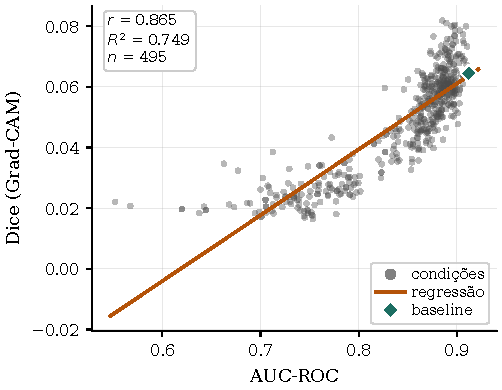
\includegraphics[width=.46\textwidth]{figura1_auc_dice}
\caption{AUC-ROC vs. Dice (Grad-CAM $\times$ lesão real) em 495 condições,
  média de 10 repetições. O losango marca o \emph{baseline} (sem filtro).}
\label{fig:scatter}
\end{figure}

A Tabela~\ref{tab:corr} reporta a mesma análise para as três métricas de
explicabilidade. O padrão é consistente nas três: correlações fortes
($r>0,83$) e altamente significativas ($p<0,001$), com o AUC-ROC explicando
entre 69\% e 75\% da variância observada em cada métrica.

\begin{table}[ht]
\centering
\caption{Correlação entre AUC-ROC e métricas de fidelidade do Grad-CAM
  ($n=495$ condições)}
\label{tab:corr}
\begin{tabular}{lccc}
\hline
\textbf{Métrica} & $r$ & $R^2$ & $p$ \\
\hline
Dice            & 0,865 & 0,749 & $<0,001$ \\
IoU             & 0,862 & 0,744 & $<0,001$ \\
Pointing Game   & 0,831 & 0,690 & $<0,001$ \\
\hline
\end{tabular}
\end{table}

A condição \emph{baseline} (sem pré-processamento) obteve AUC-ROC $=0,912$,
Dice $=0,065$, IoU $=0,036$ e Pointing Game $=0,080$ (médias de 10
repetições) -- próxima ao topo da nuvem de pontos e do previsto pela reta de
regressão para seu nível de AUC, sem se destacar como ponto fora do padrão
geral.

\textbf{Confirmação multi-método.} A Tabela~\ref{tab:multimethod} repete a
análise de correlação da Tabela~\ref{tab:corr} nas 10 condições da
subamostra, para os três métodos. Grad-CAM e LIME reproduzem a correlação
positiva forte vista nas 495 condições ($r=0,73$--$0,77$, $p<0,02$);
Occlusion Sensitivity não ($r<0,42$ em todas as métricas, $p>0,2$).

\begin{table}[ht]
\centering
\caption{Correlação AUC-ROC $\times$ fidelidade, por método ($n=10$)}
\label{tab:multimethod}
\begin{tabular}{lccc}
\hline
\textbf{Método} & Dice ($r$, $p$) & IoU ($r$, $p$) & Pointing Game ($r$, $p$) \\
\hline
Grad-CAM   & 0,76 / 0,011 & 0,75 / 0,013 & 0,77 / 0,010 \\
LIME       & 0,74 / 0,015 & 0,73 / 0,017 & 0,22 / 0,545 \\
Occlusion  & 0,08 / 0,820 & 0,10 / 0,792 & 0,42 / 0,233 \\
\hline
\end{tabular}
\end{table}

\textbf{Sanity check.} Das 29 combinações válidas condição $\times$ método
(uma indefinida por gradiente constante), 26 (90\%) mostram queda de
$\rho=1,0$ (referência) para próximo de zero conforme o modelo é
aleatorizado -- evidência de dependência real aos pesos aprendidos. A
exceção é o LIME em uma condição, cujo mapa permanece quase inalterado
($\rho=0,92$) mesmo com o modelo totalmente aleatorizado. A
Figura~\ref{fig:multimethod} ilustra os dois padrões: (A) a correlação
AUC-ROC$\times$Dice por método, com reta de regressão só para os dois
casos significativos; (B) a trajetória média de $\rho$ do sanity check por
método, com a condição em que o LIME falha destacada à parte.

\begin{figure}[ht]
\centering
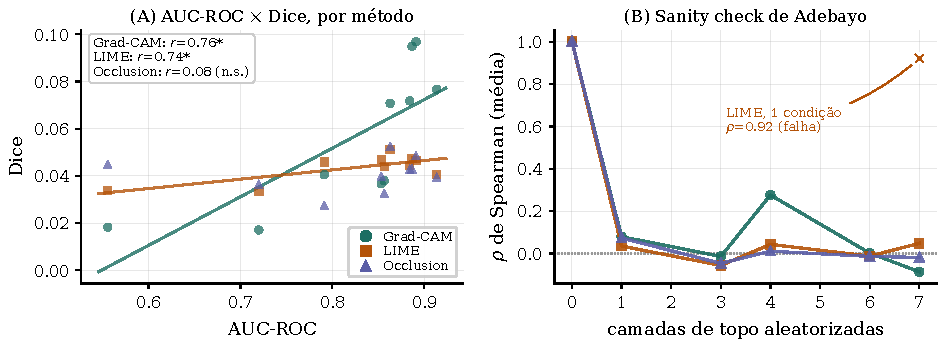
\includegraphics[width=\textwidth]{figura2_multimetodo}
\caption{Confirmação multi-método (10 condições; verde-círculo = Grad-CAM,
  laranja-quadrado = LIME, roxo-triângulo = Occlusion). (A) AUC-ROC
  $\times$ Dice, reta de regressão só nos casos significativos. (B) Sanity
  check de Adebayo, $\rho$ de Spearman médio por etapa; o X laranja marca a
  única condição em que o LIME falha.}
\label{fig:multimethod}
\end{figure}

\section{Discussão}\label{sec:discussao}

A correlação positiva forte observada nas três métricas sugere que, neste
espaço de busca, a mesma característica de imagem que ajuda o classificador
a separar as classes também ajuda o Grad-CAM a concentrar ativação sobre a
lesão real: pré-processamentos que preservam ou realçam sinal
fisiologicamente relevante (contraste local, canal verde) tendem a
favorecer ambos os objetivos, enquanto transformações mais agressivas
prejudicam os dois ao mesmo tempo. Isso é consistente com a leitura de Bell
et al.\ \cite{bell2022justnotsimple} de que o trade-off
acurácia--explicabilidade, embora real em alguns contextos, não é uma lei
geral.

A confirmação com LIME -- surrogate local, não gradiente -- torna
improvável que a correlação seja artefato específico do Grad-CAM; é
justamente essa concordância entre mecanismos independentes que a
taxonomia de Nauta et al.~\cite{nauta2023co12} chama de consistência. Já a
ausência de correlação com Occlusion Sensitivity é um limite real: seu mapa
usa uma grade de patches ($32\times32$px, passo 16) possivelmente grosseira
demais para lesões pequenas de RD, o que pode diluir a fidelidade fina
medida por Dice/IoU sem eliminar a capacidade do método de acertar a região
em termos absolutos. O sanity check de Adebayo et
al.~\cite{adebayo2018sanity} reforça esse cuidado: confirma que a maioria
das explicações depende dos pesos do modelo, mas isola exatamente o caso
(LIME, uma condição) em que essa dependência falha -- o tipo de verificação
que uma correlação agregada, sozinha, não revelaria.

\textbf{Limitações.} A correlação é observacional, não causal: não
manipulamos isoladamente o mecanismo pelo qual um filtro afeta as duas
métricas. Seguindo o alerta de Arun et al.\ \cite{arun2021trustworthiness},
Dice e IoU sobre saliência binarizada por limiar fixo não garantem que o
Grad-CAM reflita fielmente a decisão do modelo -- nossa conclusão é sobre a
variação \emph{relativa} dessas métricas, não sobre seu valor absoluto como
prova de confiabilidade clínica. O sanity check tratou o backbone
EfficientNetV2S como um único bloco (não camada a camada) -- mais
grosseiro que o protocolo original de Adebayo et al., mas suficiente para
expor o caso de falha do LIME. A subamostra multi-método tem $n=10$
condições, o que limita o poder estatístico das correlações não
significativas (Occlusion, Pointing Game do LIME) sem invalidar a
confirmação obtida com Grad-CAM e LIME. Por fim, o resultado é específico a
uma arquitetura, um conjunto de dados e uma família de transformações de
contraste/cor.

\section{Conclusão}

Em 495 condições de pré-processamento para classificação de retinopatia
diabética, acurácia (AUC-ROC) e fidelidade da explicação Grad-CAM
correlacionam-se de forma forte e positiva, contrariando a suposição de que
otimizar uma implica sacrificar a outra. Replicando a análise em uma
subamostra representativa com dois métodos mecanisticamente distintos,
confirmamos o padrão com LIME e o refutamos com Occlusion Sensitivity; um
teste de sanidade de aleatorização de modelo valida a dependência das
explicações aos pesos aprendidos na maioria dos casos, isolando uma exceção
pontual. O achado central não é específico ao Grad-CAM, mas também não é
universal a qualquer método -- distinção que avaliações de XAI em imagem
médica devem reportar. Trabalhos futuros podem testar se o padrão se
mantém em outras arquiteturas, e investigar diretamente por que Occlusion
Sensitivity diverge (ex.: variando o tamanho do patch).

\begin{thebibliography}{8}

\bibitem{selvaraju2017gradcam}
Selvaraju, R.~R., Cogswell, M., Das, A., Vedantam, R., Parikh, D., and
  Batra, D. (2017).
\newblock Grad-CAM: Visual explanations from deep networks via gradient-based
  localization.
\newblock In \emph{Proceedings of the IEEE International Conference on
  Computer Vision (ICCV)}, pages 618--626.

\bibitem{bell2022justnotsimple}
Bell, A., Solano-Kamaiko, I., Nov, O., and Stoyanovich, J. (2022).
\newblock It's just not that simple: An empirical study of the
  accuracy-explainability trade-off in machine learning for public policy.
\newblock In \emph{Proceedings of the 2022 ACM Conference on Fairness,
  Accountability, and Transparency (FAccT '22)}, pages 248--266.

\bibitem{arun2021trustworthiness}
Arun, N., Gaw, N., Singh, P., Chang, K., Aggarwal, M., Chen, B., Hoebel, K.,
  Gupta, S., Patel, J., Gidwani, M., Adebayo, J., Li, M.~D., and
  Kalpathy-Cramer, J. (2021).
\newblock Assessing the (un)trustworthiness of saliency maps for localizing
  abnormalities in medical imaging.
\newblock \emph{Radiology: Artificial Intelligence}, 3(6):e200267.

\bibitem{dash2025ocular}
Dash, S.~K., Behera, S.~K., Jena, S., Ratha, A.~K., Sethy, P.~K., and
  Nanthaamornphong, A. (2025).
\newblock Ocular disease detection using fundus images: A hybrid approach of
  Grad-CAM and multiscale Retinex preprocessing with VGG16 deep features and
  fine KNN classification.
\newblock \emph{Applied Computational Intelligence and Soft Computing},
  2025.

\bibitem{ribeiro2016lime}
Ribeiro, M.~T., Singh, S., and Guestrin, C. (2016).
\newblock ``Why should I trust you?'': Explaining the predictions of any
  classifier.
\newblock In \emph{Proceedings of the 22nd ACM SIGKDD International
  Conference on Knowledge Discovery and Data Mining (KDD)}, pages
  1135--1144.

\bibitem{zeiler2014visualizing}
Zeiler, M.~D. and Fergus, R. (2014).
\newblock Visualizing and understanding convolutional networks.
\newblock In \emph{Proceedings of the European Conference on Computer
  Vision (ECCV)}, pages 818--833.

\bibitem{adebayo2018sanity}
Adebayo, J., Gilmer, J., Muelly, M., Goodfellow, I., Hardt, M., and Kim, B.
  (2018).
\newblock Sanity checks for saliency maps.
\newblock In \emph{Advances in Neural Information Processing Systems
  (NeurIPS)}, volume~31.

\bibitem{nauta2023co12}
Nauta, M., Trienes, J., Pathak, S., Nguyen, E., Peters, M., Schmitt, Y.,
  Schlötterer, J., van Keulen, M., and Seifert, C. (2023).
\newblock From anecdotal evidence to quantitative evaluation methods: A
  systematic review on evaluating explainable AI.
\newblock \emph{ACM Computing Surveys}, 55(13s):1--42.

\end{thebibliography}

\end{document}
